
\documentclass[a4paper,10pt,article,oneside,english]{memoir} 
% DANSK OPSÆTNING
\usepackage[english]{babel}
\usepackage[utf8]{inputenc}
\usepackage[T1]{fontenc}
\usepackage{lmodern} 
\renewcommand{\englishhyphenmins}{22} 


% FIGURER
\usepackage{graphicx}

% MATEMATIK
\usepackage{amsmath}
\usepackage{amssymb,amsthm,bm}
\usepackage{mathtools}	


\begin{document}
%\frontmatter
%\clearpage	
%\tableofcontents*
	\title{Machine Learning E16 - Handin 1\\Linear classification of handwritten digits}
	\author{Mark Medum Bundgaard, Morten Jensen, Martin Sand Nielsen\\ Aarhus University}
	\date{\today}
	
	\mainmatter
	\maketitle
%\chapter{Introduction}½



\chapter{Optical Character Recognition}
A simple form of OCR to recognize handwritten digits has been achieved with linear classifiers. 

The algorithms of this exercise is programmed in Python 3.5 and Numpy by expanding the provided examples/template Jupyter Notebook.

\section{Data sets}
Two similar data sets is used for training and testing linear classifiers of handwritten digits. The first is the MNIST database\footnote{http://yann.lecun.com/exdb/mnist/} with $60000$ examples for training and $10000$ for testing. Second we have a smaller test and training set which has been written by students following the course \emph{Machine Learning} at Aarhus University through the last couple of years. We will distinguish them as the MNIST and AU data sets.


Both dataset stores each digits as a 8-bit monochrome $28\times28$ white on black image. The MNIST digits has been centered and size-normalized, which could result in more consistent results, than with the non-edited AU digits. 

The image features to be used for classification is the raw $784$ pixel values. With $n$ such sample vectors $\vec{x}_i\in \mathbb{R}^{784}$, we are given the set as a matrix, $\mathbf{X} = [x_1, x_2, \dots, x_n]^T$. For training and testing a classifier the corresponding labels $y_i \in \{0,1,\dots,9\}$ is given as the column vector $\vec{y} = [y_1, y_2, \dots, y_n]^T$. 


\chapter{Linear classification}
The linear classifier can be understood as decision-hyperplane, which can be written as $\vec{w}^T \vec{x} + w_0= 0$, where an dummy coordinate to the data vector, $x_0=1$, allow for having all the classifier parameters in one single vector $\vec{w} = [w_0, w_1, \dots, w_{784}]^T$. The equality is only true for data points that lie on the decision-surface, where points above or below will result in a negative or positive result, which can be used for classification between two classes, known as the \emph{perceptron}. 

Of course a 0-9digit OCR chould be able to distinguish all 10 classes of digits. But the simple linear classifier is still implemented for illustrative purposes on the 2's and 7's of the dataset. In a similar way this could been tried to train a one-versus-all classifier, that could tell ie. 2's from all other digits. The Softmax multiclass classifier will be introduced in section \ref{sec:softmax}.
\section{Logistic regression}
Since the perceptron-algorithm that can find the parameters of such a linear classifier is at no use when data points are not linear separable, we will try using an approach that can allow for some classification errors, but can be numerically optimized. The logistic sigmoid probability distribution and its derivative 
\begin{equation*}
\sigma(z) = \frac{1}{1+ e^{-z}}, \quad \frac{\partial \sigma(z)}{\partial z} = (1 - \sigma(z))\sigma(z)
\end{equation*}
can be used to model the target values with $\sigma(\vec{w}^T \vec{x})$. It can be found that a negative log likelihood (NLL) of the data points (digits and targets) actually come from such a distribution is given by,
\begin{equation*}
\text{NLL}(\mathbf{X},\vec{y}|\vec{w}) = - \sum_{i=1}^n y_i \ln\sigma(\vec{w}^T \vec{x}_i) + (1 - y_i)\ln\sigma(\vec{w}^T \vec{x}_i),
\end{equation*}
with the gradient 
$\frac{\partial \text{NLL}}{\partial \vec{w}}= - \mathbf{X}^T(\vec{y} - \sigma(\vec{w}^T \vec{x}))$. This NLL wil be used in a cost function, $E_{in} = \frac{1}{n}\text{NLL}$, and its gradient $\nabla E_{in} = \frac{1}{n}\frac{\partial \text{NLL}}{\partial \vec{w}}$. 



\section{Gradient descent}
The $E_{in}$ can be used to compare different learned classifier parameters $\vec{w}$ against each other. Since the cost is convex, the gradient can be used to numerically find the $\vec{w}$ (weights) that minimize cost, by iteratively moving a little downhill in the negative gradient (Gradient descent) direction ,
\begin{equation}
\vec{w}_\text{i+1} = \vec{w}_i -\eta \cdot \nabla E_{in}(\vec{w}_i).
\end{equation}
The \emph{step size} or \emph{learning rate}, $\eta$, is a positive scalar hyper parameter that can have a huge impact on training time. Too big step size could result in never converge towards minimum cost, if the algorithm is 'stepping over it'. Too small step size results in lots of iterations and unnecessary computations. It will be computational expensive to compute the cost and gradient over and over for big training sets.



\section{Stochastic gradient descent}
To improve training performance with big data sets, stochastic gradient descent (SGD), takes advantage of the fact that smaller subsets will have approximately similar cost function and gradient. So by taking just a \emph{mini batch} of the permuted full dataset to each iteration in the gradient descent algorithm, it would approximate the same weights. This of course introduces another hyper parameter, the \emph{batch size}, to our training model. When all data points have been used once, it is permuted again. A small batch size makes computation times way smaller but with increased stochastic descent towards minimum. 

We have implemented both gradient descent and SGD for a comparison in section \ref{sec:res}.




\subsection{Theoretical considerations} Since the each image pixels represents a coordinate in the 784-dimensional space, they can be permuted the same way and we would not have lost any of the information our classifiers is going to use. When training a classifier on these permuted sets, the classifier would converge towards the same weights, just permuted as well.

Furthermore we could expect that if the data set is linearly separable, the weights will be similar to those of a successful perceptron algorithm. But since the weights can be scaled with a constant without changing the decision hyperplane, they could converge towards infinity if small numerical uncertainties were to never let the gradient be exactly zero. 

Therefore regularization of the weights is explored in section \ref{sec:reg}. An additional term to the cost, that represent a penalty for large weights either as $l^1$- or $l^2$-norm, would result in a convex addition to the gradient, which would then still be convex.




\section{Softmax regression}\label{sec:softmax}
To expand the use of linear classification to a multiclass case, softmax can be used. The setup for training softmax for $K$ classes is largely similar to the logistic sigmoid. The target values are stored as a 1-of-$K$ vector, which makes the combined target matrix $\mathbb{Y}$ has shape $n \times K$. For each digit softmax computes a $K$ probabilities, one for each possible class. The digit is then classified accordingly to the highest class probability. The softmax,
\begin{equation}
\text{softmax}(\vec{x})_j = \frac{e^x_j}{\sum_{i=1}^K e^x_i}, \text{ for } j=1,\dots,K , 
\end{equation}
ensures that the sum of probabilities is always unity. This time the weights are in a matrix $\mathbf{W}$ with size $d+1 \times K$, to accomodate the $K$ classes and dummy coordinate. When modeling the target vectors with $\text{softmax}(\mathbf{w_j}^T \vec{x})$, we can find a NLL cost function,
\begin{equation}
E_\text{in} = - \frac{1}{n} \sum_{\vec{x_i}, \vec{y_i}} \vec{y_j}^T \ln\text{softmax}(\mathbf{W}^T \vec{x_j}),
\end{equation} and its gradient,
\begin{equation}
\nabla E_\text{in} = -\mathbf{X}^T \left(\mathbf{Y - softmax(\mathbf{X}\mathbf{W})}\right).
\end{equation} 
These can with just minor adjustments be used in the gradient descent and SGD algorithms used earlier.










\chapter{Results}\label{sec:res}
Below we have included some of the results achieved through the work and implementation with this exercise. Our best parameters has been saved to numpy files and handed in as well as this small report.

\section{Step size}\label{sec:stepsize}
For different values of stepsize, the higher the value, the faster we move closer to zero in cost but the gives a higher chance to overshoot the optimal cost value. 

The data is linearable seperable, so that is we have very little occilisation for different stepsizes in Figure \ref{fig:stepsize}. The red line is the only line showing oscillation, and it has a stepsize of 100, which provokes the osccilation.
\begin{figure}[h!]
	\centering
	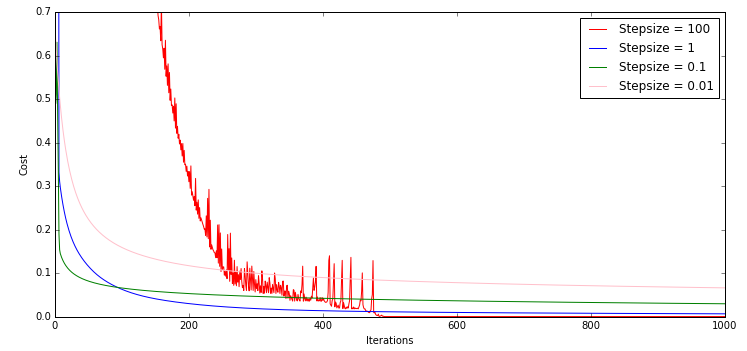
\includegraphics[width=\linewidth]{nll_plot1v2.png}
	\caption{Cost convergence for different step sizes.}
	\label{fig:stepsize}
\end{figure}





\section{Training time}
As we see in Figure \ref{fig:mini_batch} and \ref{fig:mini_batch2} the mini-batch descent obtains a good result faster, but after long enough time, the normal batch\_grad\_descent gets a better and more consistent result.
\begin{figure}[h!]
	\centering
	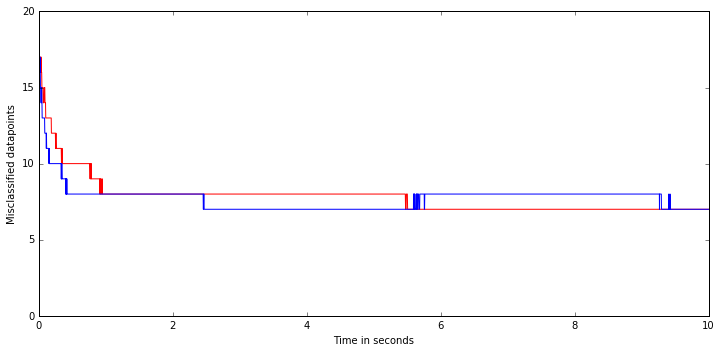
\includegraphics[width=\linewidth]{nll_plot2.png}
	\caption{Misclassifications of AUdigits vs. trainingtime. Blue is mini-batch, red is full-batch.}
	\label{fig:mini_batch}
\end{figure}
\begin{figure}[h!]
	\centering
	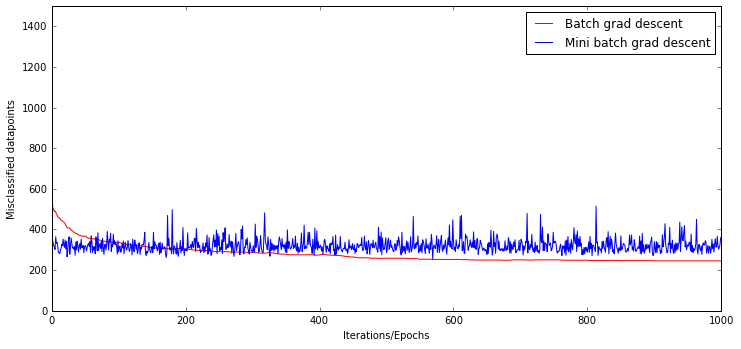
\includegraphics[width=\linewidth]{sm_plot2.png}
	\caption{Misclassifications of MNIST vs. trainingtime. }
	\label{fig:mini_batch2}
\end{figure}



\section{Classification errors}

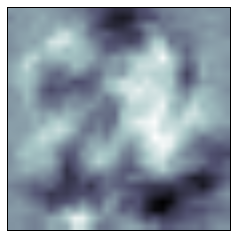
\includegraphics[scale=0.2]{nll_pict1.png}
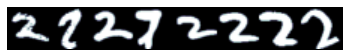
\includegraphics[scale=0.8]{nll_pict1_0.png}\\
Here you can see the visualization of the $w$ for classifying 2's and 7s from full-batch training on AUdigits. It is easy to see the dark areas where there would be a two, and the bright areas where there would be a seven. The digits are examples of misclassification. Test errors were $1.6\%$. Likewise for the mini-batch the errors were $1.6\%$, and resulted in similar weights:\\
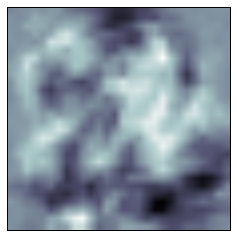
\includegraphics[scale=0.2]{nll_pict2.png}
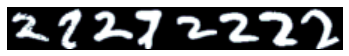
\includegraphics[scale=0.8]{nll_pict2_0.png}\\

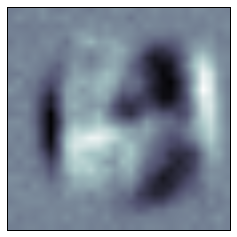
\includegraphics[width=0.2\linewidth]{nll_pict3.png}
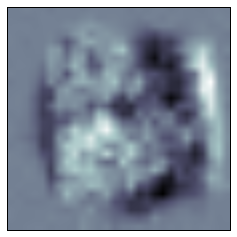
\includegraphics[width=0.2\linewidth]{nll_pict4.png}\\
Above we see the visualization of the w for classifying 2's and 7's when looking at MNIST data. The centering and size-normalization results ind the flat areas around the edges.


\noindent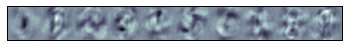
\includegraphics[width=1\linewidth]{nll_pict5.png}\\
\noindent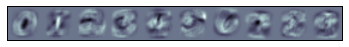
\includegraphics[width=1\linewidth]{sm_pict2.png}\\
The two images above are visualizations of the softmax weights for the numbers 0-9, for both AUdigits ($10.5\%$ errors) and MNIST ($9.8\%$ errors). Examples of misclassified digits:\\
\noindent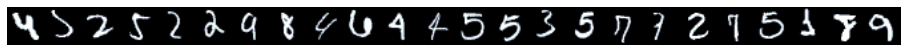
\includegraphics[width=1\linewidth]{nll_pict7_168.png}\\

\section{Regularization}\label{sec:reg}
\hspace{0.1\linewidth}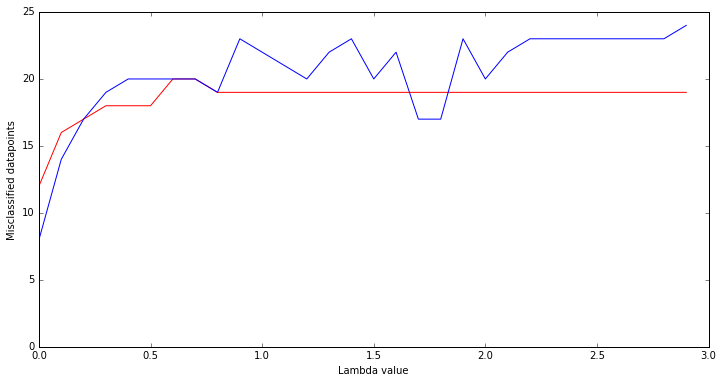
\includegraphics[width=0.8\linewidth]{nll_plot3.png}\\
Here we see a plot showing the effect of setting a lambda value between 0 and 3. In this case it is the 2's and 7's classification. As we can see, there is no gain in applying regularization. This is probably because the variance in the data is fairly small, since we only look at two different numbers.

\noindent\hspace{0.1\linewidth}
\includegraphics[width=0.8\linewidth]{nll_plot4.png}\\
Here we see a plot much like the above, but in this case, we are plotting for the One vs All classification. Here we see, that for Batch\_Grad\_Descent, we are actually improving the result, by applying regularization. This is probably because of the fact, that there is a lot more variance in the numbers that doesn't look like i, for any number $i$.



\chapter{Discussion}
Through this exercise we have found that even these simple linear classifiers, logistic sigmoid and softmax, can yield good results above $98\%$ successful classifications in the two-class case and $90\%$ in the 10 class case.

The hyper parameters for training has been the big challenge. Finding the balance between fast training and precision. Regularization has not shown to improve the general performance. 



	
\end{document}
